%%%%%%%%%%%%%%%%%%%%%%%%%%%%%%%%%%%%%%%%%%%%%%%%%%%%%%%%%%%%%%%%%%%%%%%%
%                                                                      %
%     File: Thesis_Results.tex                                         %
%     Tex Master: Thesis.tex                                           %
%                                                                      %
%     Author: Andre C. Marta                                           %
%     Last modified :  4 Mar 2024                                      %
%                                                                      %
%%%%%%%%%%%%%%%%%%%%%%%%%%%%%%%%%%%%%%%%%%%%%%%%%%%%%%%%%%%%%%%%%%%%%%%%

\chapter{Results}
\label{chapter:results}

This chapter presents the simulation scenarios considered in this work. The results obtained from the implementation presented in Chapter~\ref{chapter:implementation} are then shown and analysed, based on ideal simulations of the proposed system. As previously mentioned, the simulations and results analysed in this chapter are limited to the tethered \gls{uav} subsystem.

\section{Simulation Scenarios}
The objective is to validate the controller formulation and to assess its capability to track reference trajectories while explicitly enforcing the constraints introduced by the vehicle dynamics and by the tether.

Two simulation scenarios are considered. In the first scenario, a feasible reference trajectory is assigned to the \gls{uav}, respecting the imposed system constraints. This scenario is intended to evaluate the tracking performance of the controller and to analyse its ability to compensate for the dynamics introduced by the tether.

In the second scenario, the reference trajectory is deliberately defined such that it violates one or more system constraints. This case allows the evaluation of the controller’s ability to correctly enforce these constraints, maintaining safe operation while tracking the reference trajectory whenever feasible.

\section{Nominal Scenario Results}
\label{subsec:nominal_results}

In this scenario, a circular reference trajectory with a radius of 3~m and an altitude of 10~m was defined in the inertial reference frame. The inertial frame is oriented such that its $z$-axis points upward, facilitating the interpretation of the results.

The reference consists of a position vector $\mathbf{p}_{\mathrm{ref}}$ and a corresponding tangential velocity vector $\dot{\mathbf{p}}_{\mathrm{ref}}$ along the circular path, with a constant magnitude of 5~m/s. The UAV’s initial state is located at the origin of the inertial frame, coinciding with the anchor point.

The reference trajectory is introduced into the nonlinear programming (NLP) problem as a time-varying parameter that evolves over the prediction horizon. Each horizon therefore contains a sequence of reference values, uniformly spaced by the sampling time $T_s$.

Figure~\ref{fig:sim1_part1}(a) presents a 3D view of the UAV trajectory in the inertial frame, showing the transient phase from the initial position until the vehicle converges to and subsequently follows the prescribed circular path. Figure~\ref{fig:sim1_part1}(b) illustrates the temporal evolution of the UAV states and the corresponding reference signals.

% Figure 1: 3D and States/Inputs
\begin{figure}[H]
    \centering
    \begin{minipage}[b]{0.48\textwidth}
        \centering
        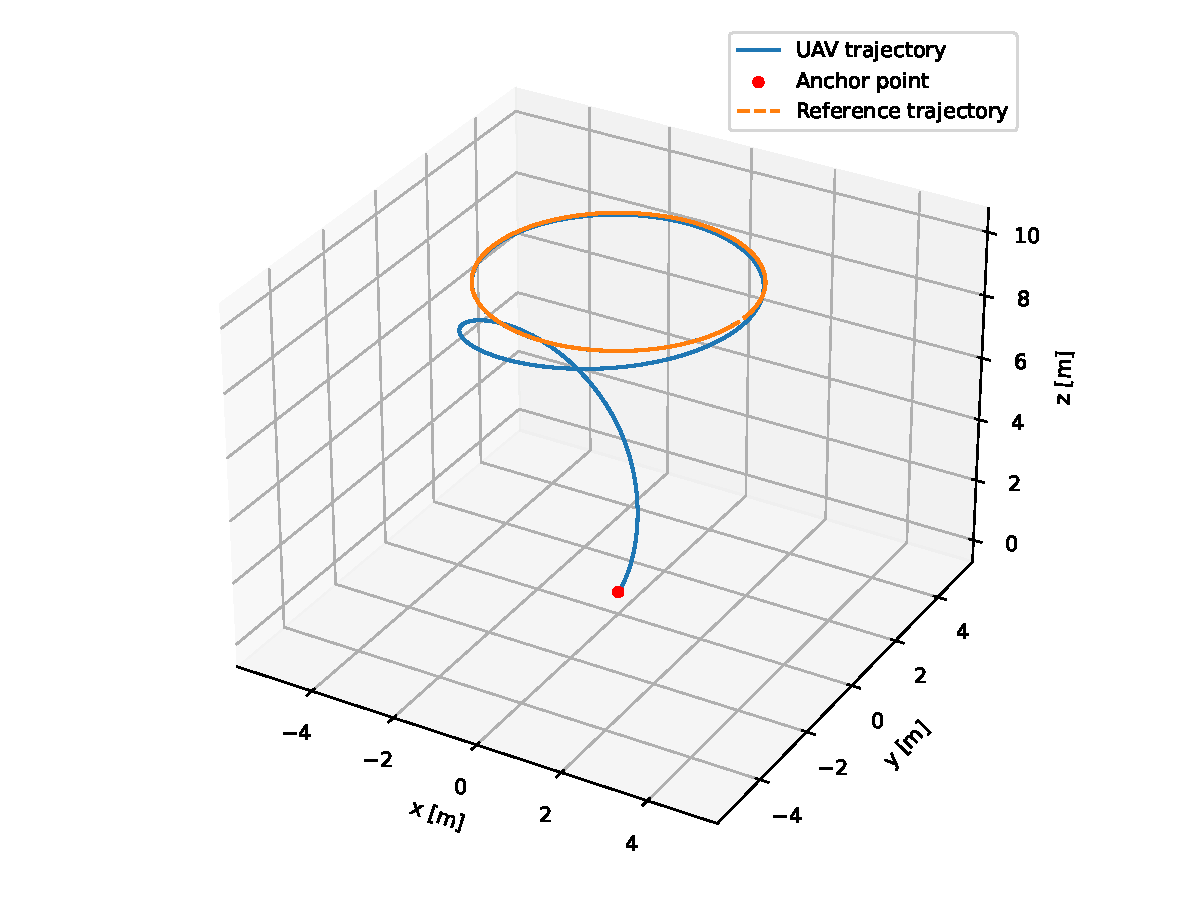
\includegraphics[width=\textwidth]{Figures/results/sim1/3d.pdf}
        \caption*{(a) UAV trajectory and reference path.}
    \end{minipage}
    \hfill
    \begin{minipage}[b]{0.48\textwidth}
        \centering
        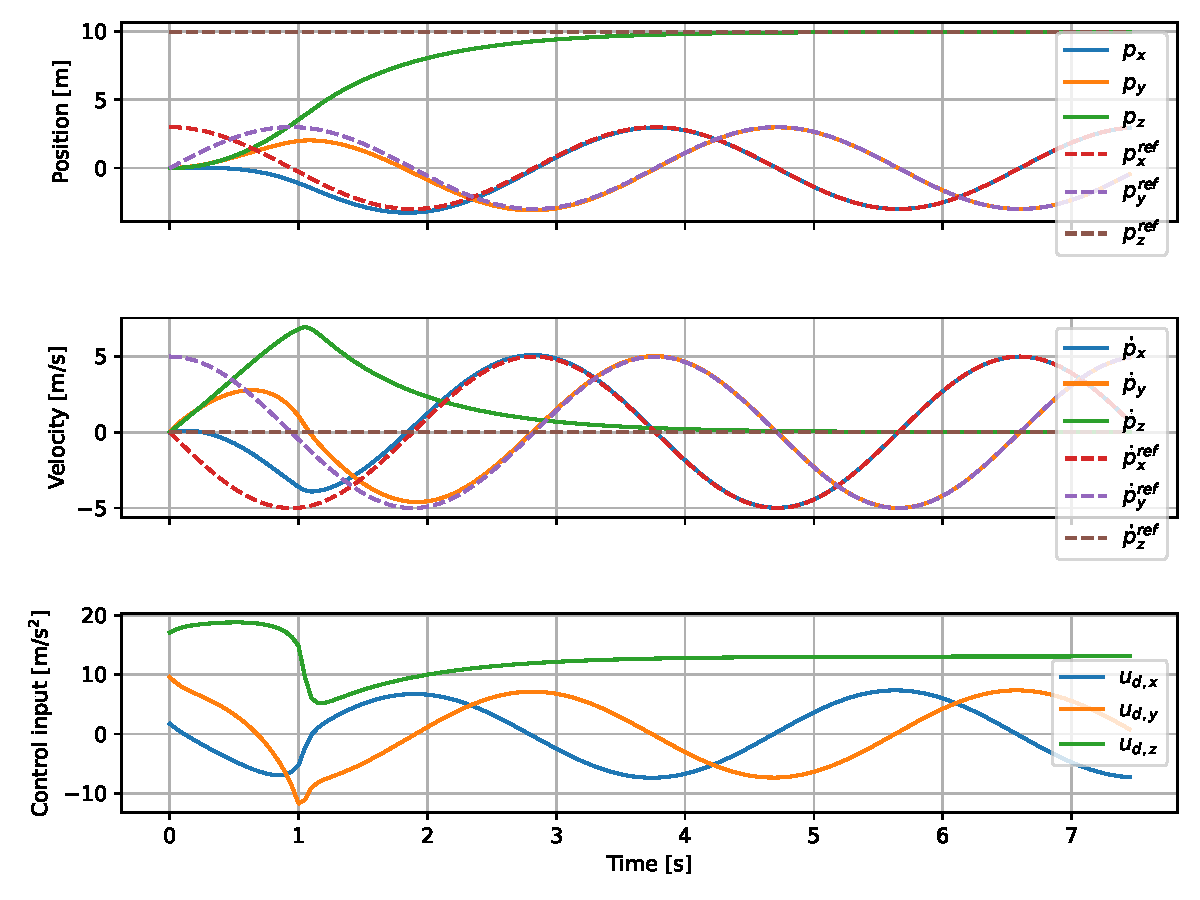
\includegraphics[width=\textwidth]{Figures/results/sim1/states_inputs.pdf}
        \caption*{(b) Position, velocity, and control inputs with their corresponding references.}
    \end{minipage}
    \caption{UAV trajectory, states, and control inputs for the nominal scenario.}
    \label{fig:sim1_part1}
\end{figure}

The plots in Figure~\ref{fig:sim1_part1}(a) evidence accurate tracking performance. Once the UAV reaches the desired altitude, all state variables converge to their respective references, as expected.  

The inertial acceleration components $u_{d,(x,y,z)}$ responsible for this tracking performance show oscillations in the $x$ and $y$ components due to attitude variations that adjust the thrust direction and enable the UAV to follow the reference trajectory, while the $z$ component stabilises at a value that compensates for gravity and the vertical force imposed by the tether.


Figure~\ref{fig:sim1_part2}(a) shows the components of the acceleration induced by the tether on the UAV $a_{\text{tether}}$, as well as the total inertial acceleration $\ddot{\mathbf{p}}$, as a function of time.  
Figure~\ref{fig:sim1_part2}(b) presents the three imposed constraints, the maximum tether length $L_{\text{max}}$, the maximum velocity $\|\dot{\mathbf{p}}\|_{\text{max}}$, and the maximum control acceleration $\|u_d\|_{\text{max}}$, together with their respective constrained variables.


% Figure 2: Acc and Modules
\begin{figure}[H]
    \centering
    \begin{minipage}[b]{0.48\textwidth}
        \centering
        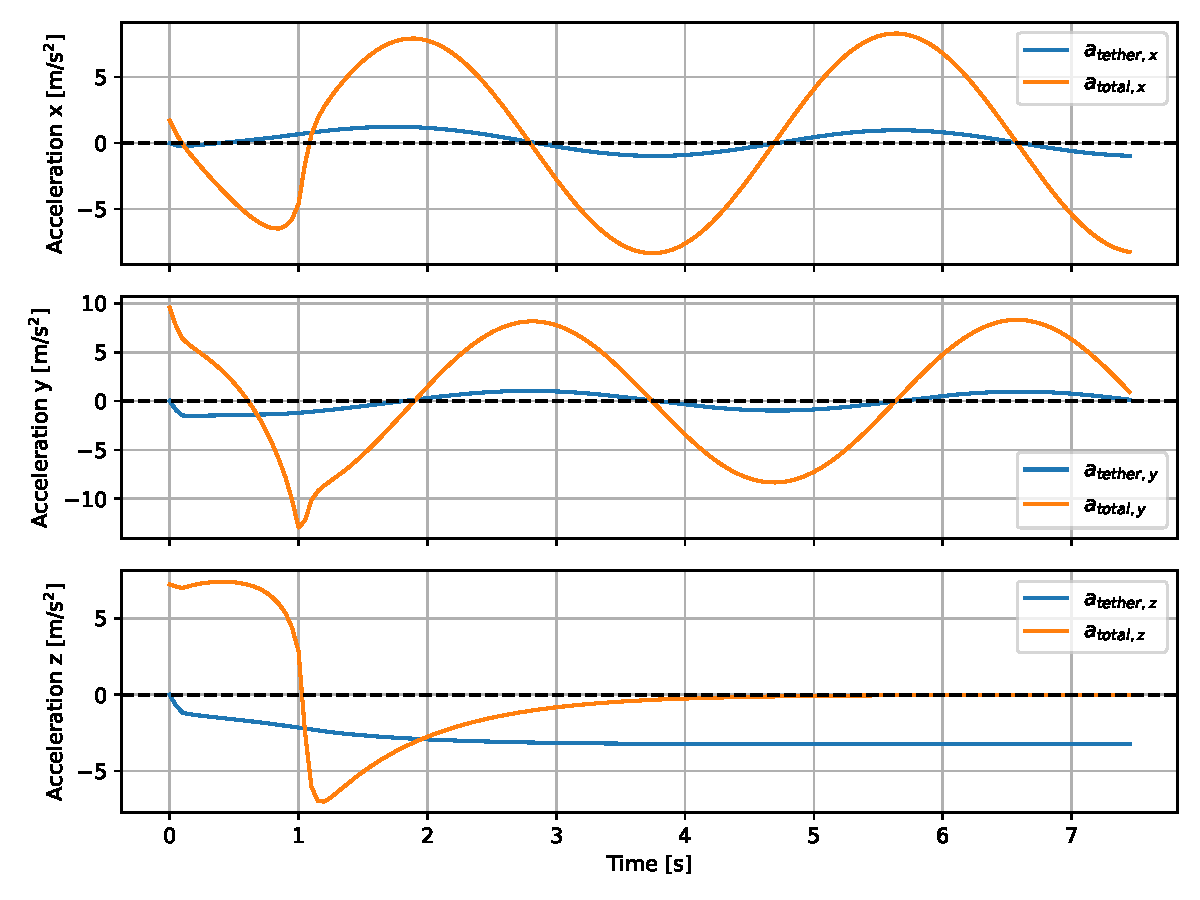
\includegraphics[width=\textwidth]{Figures/results/sim1/acc.pdf}
        \caption*{(a) Total and tether-induced acceleration components.}
    \end{minipage}
    \hfill
    \begin{minipage}[b]{0.48\textwidth}
        \centering
        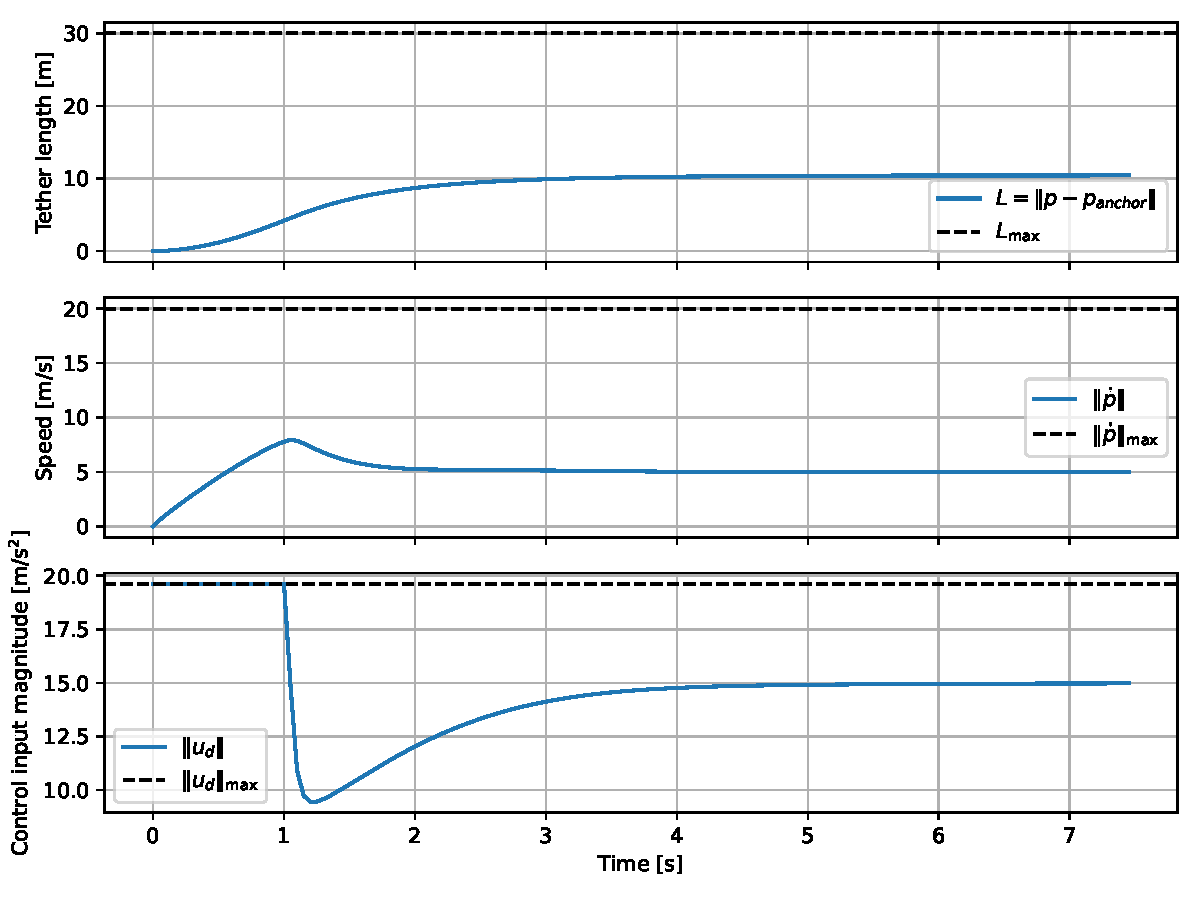
\includegraphics[width=\textwidth]{Figures/results/sim1/modules.pdf}
        \caption*{(b) Tether length, speed, and control acceleration magnitudes with respective constraints.}
    \end{minipage}
    \caption{Acceleration and constraint magnitudes for the nominal scenario.}
    \label{fig:sim1_part2}
\end{figure}

The $z$-component of the tether acceleration, $a_{\text{tether},z}$, increases as the tether extends from the anchor point until reaching the trajectory height of 10~m, since the tether is modelled as a force that grows with the UAV’s distance from the anchor point.  
As expected, $\ddot{\mathbf{p}}_z$ converges to zero as the UAV maintains a constant altitude, while $\ddot{\mathbf{p}}_x$ and $\ddot{\mathbf{p}}_y$ exhibit oscillations due to the circular motion.

It can be observed that only the control acceleration magnitude, $\|u_d\| = T/m$, reached and respected its constraint of $2g$, stabilising once the UAV achieved a constant speed.  
This indicates that the thrust magnitude remained constant, while only its direction changed to follow the reference trajectory, as shown in Figure~\ref{fig:sim1_part1}(b).  
The tether length $L$ slightly exceeded 10~m, remaining well below its maximum value of 30~m, consistent with the defined trajectory, while the UAV’s speed $\|\dot{\mathbf{p}}\|$ stabilised around 5~m/s, matching the reference.


\section{Constraint-Violating Scenario Results}
\label{subsec:constraint_results}

In this scenario, the same circular trajectory was defined; however, its centre was shifted approximately 30~m away from the anchor point. As a result, part of the reference trajectory deliberately exceeded the reachable region imposed by the maximum tether length of 30~m, testing whether the constraint was properly enforced by the controller.

Figure~\ref{fig:sim2_part1}(a) shows the UAV trajectory and the reference path for the constraint-violating scenario, while Figure~\ref{fig:sim2_part1}(b) presents the corresponding state and control input evolution.

% Figure 1: 3D and States/Inputs
\begin{figure}[H]
    \centering
    \begin{minipage}[b]{0.48\textwidth}
        \centering
        
\includegraphics[width=\textwidth]{Figures/results/sim2/3d.pdf}
        \caption*{(a) UAV trajectory and reference path.}
    \end{minipage}
    \hfill
    \begin{minipage}[b]{0.48\textwidth}
        \centering
        
\includegraphics[width=\textwidth]{Figures/results/sim2/states_inputs.pdf}
        \caption*{(b) Position, velocity, and control inputs with their corresponding references.}
    \end{minipage}
    \caption{UAV trajectory, states, and control inputs for the constraint-violating scenario.}
    \label{fig:sim2_part1}
\end{figure}

It can be observed that only a portion of the trajectory closer to the anchor point was accurately followed.  
Figure~\ref{fig:sim2_part1}(b) shows that the UAV successfully sacrificed some tracking accuracy, particularly along the $x$ and $z$ axes, to satisfy the tether-length constraint.  
The corresponding control input $\mathbf{u}_d$ responsible for this motion reflects these adjustments, keeping a similar $y$ component to the previous simulation and adapting the $x$ and $z$ components.

Figure~\ref{fig:sim2_part2}(a) shows the total and tether-induced acceleration components for the constraint-violating scenario, while Figure~\ref{fig:sim2_part2}(b) presents the corresponding constraint magnitudes.

% Figure 2: Acc and Modules
\begin{figure}[H]
    \centering
    \begin{minipage}[b]{0.48\textwidth}
        \centering
        
\includegraphics[width=\textwidth]{Figures/results/sim2/acc.pdf}
        \caption*{(a) Total and tether-induced acceleration components.}
    \end{minipage}
    \hfill
    \begin{minipage}[b]{0.48\textwidth}
        \centering
        
\includegraphics[width=\textwidth]{Figures/results/sim2/modules.pdf}
        \caption*{(b) Tether length, speed, and control acceleration magnitudes with respective constraints.}
    \end{minipage}
    \caption{Acceleration and constraint magnitudes for the constraint-violating scenario.}
    \label{fig:sim2_part2}
\end{figure}

In Figure~\ref{fig:sim2_part2}(a), the acceleration along the $y$-axis remains similar to that of the nominal scenario, while the $x$ and $z$ components adapt to the imposed constraint.  
Figure~\ref{fig:sim2_part2}(b) clearly shows the tether length reaching its upper bound of 30~m without ever exceeding it, demonstrating that the constraint was correctly formulated and effectively enforced throughout the simulation.


\section{Tracking Accuracy}
\label{subsec:tracking_accuracy}

The tracking performance of the controller is analysed by comparing the UAV states with their respective references, defined as
\[
\mathbf{e}_p = \mathbf{p} - \mathbf{p}_{\text{ref}}, \qquad
\mathbf{e}_{\dot{p}} = \dot{\mathbf{p}} - \dot{\mathbf{p}}_{\text{ref}}.
\]

Figure~\ref{fig:tracking_error}(a) shows the tracking error for position and velocity components when the reference trajectory lies within the reachable zone, while Figure~\ref{fig:tracking_error}(b) presents the same quantities for the scenario where the reference trajectory extends beyond the tether’s maximum length.

% Figure: Tracking errors comparison
\begin{figure}[H]
    \centering
    \begin{minipage}[b]{0.48\textwidth}
        \centering
        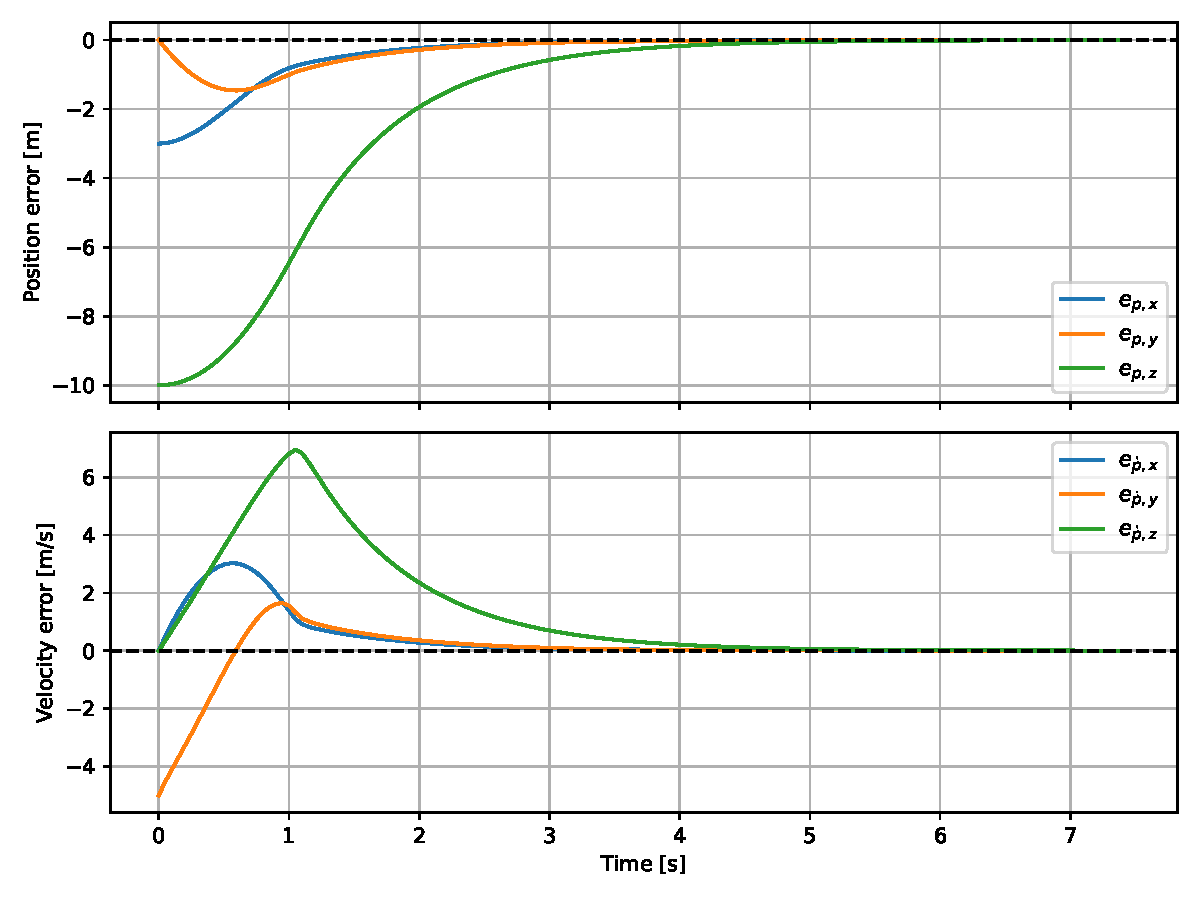
\includegraphics[width=\textwidth]{Figures/results/sim1/errors.pdf}
        \caption*{(a) Tracking error for the trajectory within the reachable zone.}
    \end{minipage}
    \hfill
    \begin{minipage}[b]{0.48\textwidth}
        \centering
        
\includegraphics[width=\textwidth]{Figures/results/sim2/errors.pdf}
        \caption*{(b) Tracking error for the trajectory outside the reachable zone.}
    \end{minipage}
    \caption{Tracking error for position and velocity states.}
    \label{fig:tracking_error}
\end{figure}

As shown in Figure~\ref{fig:tracking_error}(a), after the UAV reaches the desired trajectory, approximately between $t = 5~\text{s}$ and $t = 6~\text{s}$, the tracking errors converge to near-zero values, demonstrating the controller’s effectiveness in accurately following the reference trajectory.
 

In Figure~\ref{fig:tracking_error}(b), as previously observed, the $y$ component remains close to the reference, while the $x$ and $z$ components lose accuracy to maintain the trajectory within the tether’s reachable region. This behaviour occurs because the trajectory centre was only shifted along the $x$ and $z$ axes, allowing the $y$ component to achieve similar values to those of the nominal case while respecting the imposed constraints.

